\documentclass[tikz,border=2pt]{standalone}
\usepackage{amsmath}
\usepackage{pgfplots}
\pgfplotsset{compat=1.18}
\usetikzlibrary{arrows.meta}
\begin{document}
% Example 5.1 and its dual: (P) max 3x1+5x2, A rows (1,0),(0,2),(3,2), b=(4,12,18), x>=0;
% (D) min 4y1+12y2+18y3, A^T rows (1,0,3),(0,2,2), c=(3,5), y>=0. Rows of A become columns of A^T, b and c swap roles.
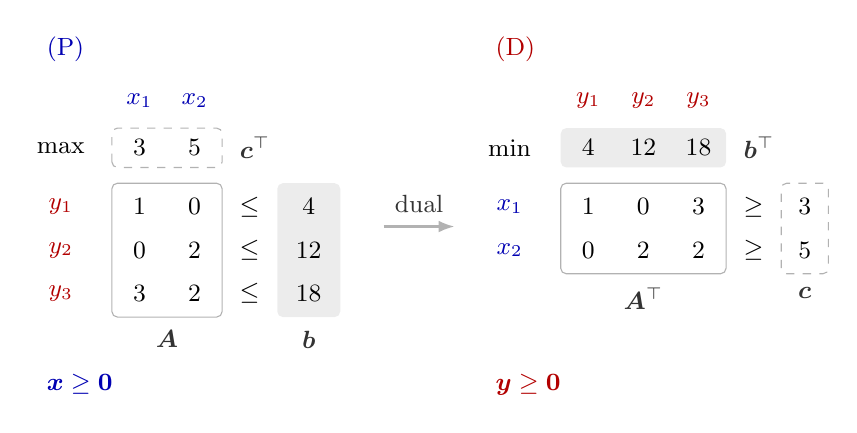
\begin{tikzpicture}[font=\small, >={Latex[length=2mm]}]
  % ---------------- primal (P) ----------------
  \begin{scope}
    \node[blue!70!black, anchor=west] at (-0.3,1.25) {(P)};
    % column headers: primal variables
    \node[blue!70!black] at (1.0,0.6) {$x_1$};
    \node[blue!70!black] at (1.7,0.6) {$x_2$};
    % objective row c^T
    \draw[gray!60, dashed, rounded corners=2pt] (0.65,-0.25) rectangle (2.05,0.25);
    \node at (0,0) {$\max$};
    \node at (1.0,0) {$3$};
    \node at (1.7,0) {$5$};
    \node[gray!40!black, anchor=west] at (2.15,0) {$\boldsymbol{c}^{\top}$};
    % constraint rows, one dual variable per row
    \draw[gray!60, rounded corners=2pt] (0.65,-2.15) rectangle (2.05,-0.45);
    \fill[gray!15, rounded corners=2pt] (2.75,-2.15) rectangle (3.55,-0.45);
    \foreach \r/\a/\b/\rhs [count=\i] in {-0.75/1/0/4, -1.3/0/2/12, -1.85/3/2/18} {
      \node[red!70!black] at (0,\r) {$y_{\i}$};
      \node at (1.0,\r) {$\a$};
      \node at (1.7,\r) {$\b$};
      \node at (2.4,\r) {$\leq$};
      \node at (3.15,\r) {$\rhs$};
    }
    \node[gray!40!black, anchor=north] at (1.35,-2.2) {$\boldsymbol{A}$};
    \node[gray!40!black, anchor=north] at (3.15,-2.2) {$\boldsymbol{b}$};
    \node[blue!70!black, anchor=north west] at (-0.3,-2.75) {$\boldsymbol{x}\geq\boldsymbol{0}$};
  \end{scope}
  % ---------------- arrow ----------------
  \draw[gray!60, ->, thick] (4.1,-1.0) -- (5.0,-1.0);
  \node[gray!40!black, anchor=south] at (4.55,-0.95) {dual};
  % ---------------- dual (D) ----------------
  \begin{scope}[xshift=5.7cm]
    \node[red!70!black, anchor=west] at (-0.3,1.25) {(D)};
    % column headers: dual variables
    \node[red!70!black] at (1.0,0.6) {$y_1$};
    \node[red!70!black] at (1.7,0.6) {$y_2$};
    \node[red!70!black] at (2.4,0.6) {$y_3$};
    % objective row b^T
    \fill[gray!15, rounded corners=2pt] (0.65,-0.25) rectangle (2.75,0.25);
    \node at (0,0) {$\min$};
    \node at (1.0,0) {$4$};
    \node at (1.7,0) {$12$};
    \node at (2.4,0) {$18$};
    \node[gray!40!black, anchor=west] at (2.85,0) {$\boldsymbol{b}^{\top}$};
    % constraint rows, one per primal variable
    \draw[gray!60, rounded corners=2pt] (0.65,-1.6) rectangle (2.75,-0.45);
    \draw[gray!60, dashed, rounded corners=2pt] (3.45,-1.6) rectangle (4.05,-0.45);
    \foreach \r/\a/\b/\cc/\rhs [count=\j] in {-0.75/1/0/3/3, -1.3/0/2/2/5} {
      \node[blue!70!black] at (0,\r) {$x_{\j}$};
      \node at (1.0,\r) {$\a$};
      \node at (1.7,\r) {$\b$};
      \node at (2.4,\r) {$\cc$};
      \node at (3.1,\r) {$\geq$};
      \node at (3.75,\r) {$\rhs$};
    }
    \node[gray!40!black, anchor=north] at (1.7,-1.65) {$\boldsymbol{A}^{\top}$};
    \node[gray!40!black, anchor=north] at (3.75,-1.65) {$\boldsymbol{c}$};
    \node[red!70!black, anchor=north west] at (-0.3,-2.75) {$\boldsymbol{y}\geq\boldsymbol{0}$};
  \end{scope}
\end{tikzpicture}
\end{document}
